\FloatBarrier
\section{Weight-space diagnostics and numerical checks}
\label{app:landscape}
The geometry study uses twenty separately trained reference models: plain, R, G and RG at seeds 0--4. Initial weights and data order are paired within each seed. All new amplitude, temporal and Hessian evaluations reuse those checkpoints; no additional optimization is needed for these diagnostics. The five-seed batch is separate from the three-seed selection batch, so its repeated seed labels do not justify pooling the runs.
% GENERATED by paper/tools/build_assets.py from data/records/ -- do not edit by hand.
% Regenerate: py paper/tools/build_records.py && py paper/tools/build_assets.py
\begin{table}[!t]
\caption{Endpoints of the separate five-seed landscape batch: CIFAR-10 / ResNet-20-BN / SGD, 30 epochs, saved BatchNorm. Accuracy uses all 10k test images; CE uses all 50k training or 10k test images. Mean $\pm$ sample SD. Bold accuracy means exceed Plain; this batch is not pooled with Table~\ref{tab:transfer}.}\label{tab:landscape-endpoints}
\centering\small\setlength{\tabcolsep}{4pt}\renewcommand{\arraystretch}{1.08}
\begin{tabular*}{\linewidth}{@{\extracolsep{\fill}}lrrr@{}}
\toprule
Method & \multicolumn{1}{c}{Test accuracy (\%)} & \multicolumn{1}{c}{Train CE (nats)} & \multicolumn{1}{c}{Test CE (nats)}\\
\midrule
Plain & $75.65\pm0.78$ & $0.197\pm0.019$ & $0.759\pm0.010$\\
Resolution & $\mathbf{80.21}\pm0.36$ & $0.303\pm0.008$ & $0.584\pm0.010$\\
Gaussian & $\mathbf{80.12}\pm0.49$ & $0.273\pm0.006$ & $0.587\pm0.021$\\
Combined & $\mathbf{81.58}\pm0.30$ & $0.312\pm0.006$ & $0.542\pm0.005$\\
\bottomrule
\end{tabular*}
\end{table}


\subsection{Evaluation sets and normalization}
The training and test probes each contain 1,000 fixed, class-balanced examples. Calibration uses a fixed 2,000-image training subset, disjoint from the training probe, in four batches of 500. Larger finite-sensitivity checks use 10,000 training images and the full test set; the larger training subset includes the training probe but is disjoint from calibration. Calibration resets running statistics and accumulates their cumulative batch averages without gradient updates. Evaluation then uses these buffers in eval mode. No test examples calibrate BatchNorm, and previous grid points do not leave their buffers in the next evaluation.

Writing $b$ for the BatchNorm buffers and $\widehat b(\theta)$ for this calibration procedure clarifies the three functions measured:
\[
 L_{\rm saved}(\theta)=L(\theta;b_{\rm checkpoint}),\qquad
 L_{\rm centre}(\theta)=L(\theta;\widehat b(\theta_0)),\qquad
 L_{\rm point}(\theta)=L(\theta;\widehat b(\theta)).
\]
The calibration batch size, order and procedure are part of the definition of $\widehat b$; it is not an exact population statistic. In centre-frozen evaluations, $\theta_0$ is the checkpoint about which the plot or derivative is computed. Saved and centre-frozen policies keep the buffers constant under weight perturbations. Pointwise recalibration includes their change. At intermediate checkpoints, the intervention state is also specified independently of the buffers.

\subsection{Direction sampling, aggregation and amplitudes}
The perturbed vector contains 268,336 convolution and classifier weights, arranged in 698 output-filter or classifier-row blocks. Biases and BatchNorm affine parameters are fixed. Every measured block has a nonzero norm. Gaussian draws are generated deterministically, shared across methods within a seed, and normalized as in Equation~\eqref{eq:direction}. One useful displacement scale is
\[
 r(\delta)=\left(\frac1{698}\sum_j\frac{\|\delta_j\|_2^2}{\|\theta_j\|_2^2}\right)^{1/2}.
\]
For the random directions, $r(\varepsilon d)=|\varepsilon|$. Directions normalized using different checkpoints need not have the same physical length or span the same plane.

The amplitudes are $0.005,0.01,0.02,0.025,0.05,0.1,0.2,0.25,0.35,0.5$. Twenty directions per model give $20\times20\times3\times2\times10=24{,}000$ directional sensitivity values across networks, policies, probes and amplitudes. We first average over directions within a checkpoint, then pair each method with plain in that seed, and only then average across the five seeds. Repeated directions and amplitudes do not increase the number of independent training replications. Sample SDs over seeds are descriptive spreads, not confidence intervals or hypothesis tests.

For a twice differentiable fixed function and a sufficiently small displacement,
\[
 \frac{2S_\theta(\varepsilon)}{\varepsilon^2}
 \longrightarrow \frac1K\sum_k d_k^\top H d_k.
\]
The symmetric evaluation cancels the first-order term. At finite amplitudes, ReLU activation changes and nonquadratic terms can invalidate that approximation; pointwise recalibration also changes the function. We therefore call $S$ a finite sensitivity, not a Hessian eigenvalue or a universal flatness measure.
% GENERATED by paper/tools/build_assets.py from data/records/ -- do not edit by hand.
% Regenerate: py paper/tools/build_records.py && py paper/tools/build_assets.py
\begin{table}[!t]
\caption{Finite sensitivity $S$ (nats) on larger evaluation sets. CIFAR-10, ResNet-20-BN/ReLU, SGD, final 30-epoch checkpoints of the five-seed landscape batch. Entries are means $\pm$ sample SD across seeds, each averaging 20 directions. $S$ is the centre-subtracted CE increase in Equation~\eqref{eq:sensitivity}, not the unperturbed loss.}\label{tab:sensitivity-validation}
\centering\small\setlength{\tabcolsep}{4pt}\renewcommand{\arraystretch}{1.08}
\begin{tabular*}{\linewidth}{@{\extracolsep{\fill}}lrrrrr@{}}
\toprule
Evaluation set & \multicolumn{1}{c}{$\varepsilon$} & \multicolumn{1}{c}{Plain} & \multicolumn{1}{c}{R} & \multicolumn{1}{c}{G} & \multicolumn{1}{c}{RG}\\
\midrule
\addlinespace[4pt]\multicolumn{6}{@{}l@{}}{\textit{Saved BatchNorm statistics}}\\[2pt]
Train subset (10k) & 0.1 & $0.732\pm0.060$ & $0.468\pm0.028$ & $0.726\pm0.086$ & $0.431\pm0.044$\\
Train subset (10k) & 0.25 & $5.269\pm0.356$ & $3.815\pm0.294$ & $4.423\pm0.184$ & $3.528\pm0.319$\\
Full test set (10k) & 0.1 & $0.625\pm0.054$ & $0.407\pm0.027$ & $0.633\pm0.082$ & $0.386\pm0.039$\\
Full test set (10k) & 0.25 & $4.866\pm0.360$ & $3.616\pm0.283$ & $4.170\pm0.199$ & $3.370\pm0.312$\\
\addlinespace[4pt]\multicolumn{6}{@{}l@{}}{\textit{BatchNorm recalibrated at each point}}\\[2pt]
Train subset (10k) & 0.1 & $0.192\pm0.015$ & $0.135\pm0.005$ & $0.283\pm0.048$ & $0.128\pm0.025$\\
Train subset (10k) & 0.25 & $1.020\pm0.067$ & $0.769\pm0.022$ & $1.283\pm0.120$ & $0.729\pm0.098$\\
Full test set (10k) & 0.1 & $0.102\pm0.009$ & $0.089\pm0.004$ & $0.213\pm0.043$ & $0.092\pm0.023$\\
Full test set (10k) & 0.25 & $0.700\pm0.061$ & $0.616\pm0.022$ & $1.079\pm0.119$ & $0.607\pm0.096$\\
\bottomrule
\end{tabular*}
\end{table}

% GENERATED by paper/tools/build_assets.py from data/records/ -- do not edit by hand.
% Regenerate: py paper/tools/build_records.py && py paper/tools/build_assets.py
\begin{table}[!htbp]
\caption{Paired differences $S_{\rm method}-S_{\rm plain}$ (nats), mean $\pm$ sample SD over five seeds. Superscripts count negative seed pairs. The populations and protocols are those of Table~\ref{tab:sensitivity-validation}.}\label{tab:sensitivity-validation-paired}
\centering\small\setlength{\tabcolsep}{4pt}\renewcommand{\arraystretch}{1.08}
\begin{tabular*}{\linewidth}{@{\extracolsep{\fill}}lrrrr@{}}
\toprule
Evaluation set & \multicolumn{1}{c}{$\varepsilon$} & \multicolumn{1}{c}{$\Delta S$: R} & \multicolumn{1}{c}{$\Delta S$: G} & \multicolumn{1}{c}{$\Delta S$: RG}\\
\midrule
\addlinespace[4pt]\multicolumn{5}{@{}l@{}}{\textit{Saved BatchNorm statistics}}\\[2pt]
Train subset (10k) & 0.1 & $-0.264\pm0.045$\,\textsuperscript{5/5} & $-0.006\pm0.111$\,\textsuperscript{3/5} & $-0.301\pm0.045$\,\textsuperscript{5/5}\\
Train subset (10k) & 0.25 & $-1.454\pm0.237$\,\textsuperscript{5/5} & $-0.846\pm0.404$\,\textsuperscript{5/5} & $-1.741\pm0.355$\,\textsuperscript{5/5}\\
Full test set (10k) & 0.1 & $-0.218\pm0.041$\,\textsuperscript{5/5} & $+0.008\pm0.108$\,\textsuperscript{2/5} & $-0.239\pm0.043$\,\textsuperscript{5/5}\\
Full test set (10k) & 0.25 & $-1.250\pm0.246$\,\textsuperscript{5/5} & $-0.696\pm0.412$\,\textsuperscript{5/5} & $-1.496\pm0.355$\,\textsuperscript{5/5}\\
\addlinespace[4pt]\multicolumn{5}{@{}l@{}}{\textit{BatchNorm recalibrated at each point}}\\[2pt]
Train subset (10k) & 0.1 & $-0.057\pm0.014$\,\textsuperscript{5/5} & $+0.091\pm0.047$\,\textsuperscript{0/5} & $-0.064\pm0.024$\,\textsuperscript{5/5}\\
Train subset (10k) & 0.25 & $-0.250\pm0.059$\,\textsuperscript{5/5} & $+0.264\pm0.126$\,\textsuperscript{0/5} & $-0.291\pm0.099$\,\textsuperscript{5/5}\\
Full test set (10k) & 0.1 & $-0.013\pm0.008$\,\textsuperscript{5/5} & $+0.110\pm0.043$\,\textsuperscript{0/5} & $-0.011\pm0.021$\,\textsuperscript{4/5}\\
Full test set (10k) & 0.25 & $-0.084\pm0.057$\,\textsuperscript{5/5} & $+0.379\pm0.130$\,\textsuperscript{0/5} & $-0.093\pm0.102$\,\textsuperscript{4/5}\\
\bottomrule
\end{tabular*}
\end{table}

\begin{figure}[htbp]\centering
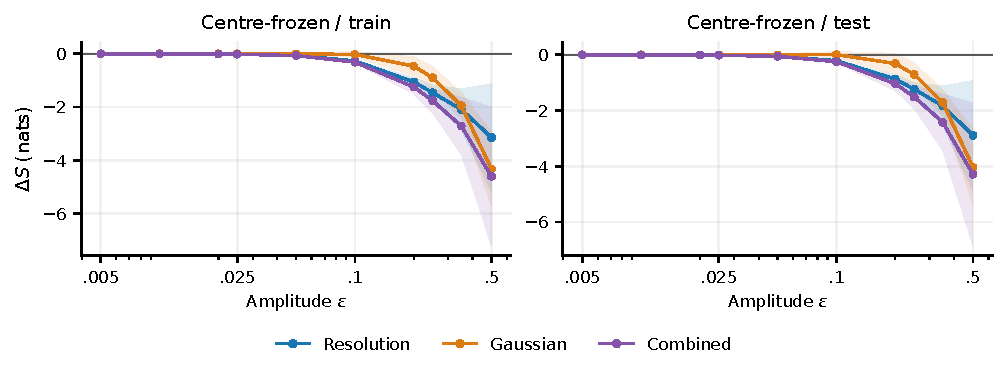
\includegraphics[width=.92\linewidth]{figures/sensitivity_centre_frozen.pdf}
\caption{The centre-frozen policy, using the same conventions as Figure~\ref{fig:sensitivity}. R and RG have negative paired differences at every amplitude in every seed on both probes. G does not share that full pattern.}
\label{fig:centre-frozen}
\end{figure}

\subsection{What the surfaces show}
A random plane evaluates $L(\theta_0+a d_1+b d_2)$ on a grid. The axes are two chosen directions in parameter space; they are not coordinates of input images. An absolute surface displays the CE itself. A centred surface displays $L(\theta_0+a d_1+b d_2)-L(\theta_0)$, so every centre has height zero even though the quoted centre CEs differ. This removes the vertical offset, not the shape. The smooth bowl-like appearance of a sampled plane does not establish convexity in all parameter directions.
Figure~\ref{fig:wide-surfaces} in the main text shows the final seed-0 planes with pointwise recalibration, using the same viewing angle, axis limits and colour scale for every method. The surfaces join all 41-by-41 measured vertices; no additional training seeds are represented by the plane.


\subsection{Hessian definitions and convergence}
\label{app:hessian-checks}
The Hessian is that of mean CE, excluding weight decay, on the selected weight subset at the final checkpoint. The ordinary operator is $H=\nabla^2_\theta L$. For block-relative coordinates, $\theta=\theta_0+Aq$ with $A_j=\|\theta_{0,j}\|_2 I$, we use $H_{\rm rel}=A^\top H A$ and keep $A$ fixed during differentiation. Normalizing by filter norms reduces an obvious scale mismatch but does not give invariance to arbitrary reparameterizations \citep{dinh2017sharp}. It also does not make the random directions isotropic in relative coordinates: their block covariance includes a factor inverse to block dimension. Random-direction averages and extreme eigenvalues answer different questions.

Hessian--vector products are computed by differentiating the loss gradient, accumulated with correct sample weights. Lanczos uses full reorthogonalization and two deterministic starts for each of 160 problems (twenty networks, two probes, two fixed-statistics policies and two coordinate choices). Each requested eigenpair must satisfy an explicit residual criterion of the form
\[
 \|Hv-\lambda v\|_2\le10^{-3}
 \max\{|\lambda|,10^{-3}|\lambda_{\max}|\},\qquad \|v\|_2=1,
\]
with $H$ replaced by $H_{\rm rel}$ when appropriate. All \tHessProblems{} problems met the criterion for the two largest and the smallest algebraic eigenvalue, from both starts; they required \tHessIterMin--\tHessIterMax{} iterations. The largest recorded relative residual is $\tHessResidTop\times10^{-7}$ for the two leading eigenpairs and $\tHessResidMin\times10^{-4}$ for the minimum eigenpair. Residuals assess the numerical eigenproblem, not whether the checkpoint is a local optimum.
% GENERATED by paper/tools/build_assets.py from data/records/ -- do not edit by hand.
% Regenerate: py paper/tools/build_records.py && py paper/tools/build_assets.py
\begin{table}[!t]
\caption{Largest algebraic Hessian eigenvalue, mean $\pm$ sample SD over five seeds. CIFAR-10 / ResNet-20-BN / SGD, 30 epochs; CE on 1k-image probes and 268\,336 convolution/classifier weights. Coordinate groups define different matrices; compare methods within rows.}\label{tab:hessian-all}
\centering\small\setlength{\tabcolsep}{4pt}\renewcommand{\arraystretch}{1.08}
\begin{tabular*}{\linewidth}{@{\extracolsep{\fill}}llrrrr@{}}
\toprule
BatchNorm policy & Probe & \multicolumn{1}{c}{Plain} & \multicolumn{1}{c}{R} & \multicolumn{1}{c}{G} & \multicolumn{1}{c}{RG}\\
\midrule
\addlinespace[4pt]\multicolumn{6}{@{}l@{}}{\textit{Ordinary parameter coordinates}}\\[2pt]
Saved & Train & $2382\pm147$ & $1444\pm100$ & $1281\pm116$ & $1148\pm56$\\
Saved & Test & $3237\pm324$ & $1677\pm77$ & $1500\pm120$ & $1282\pm59$\\
Centre-frozen & Train & $2354\pm160$ & $1438\pm107$ & $1275\pm128$ & $1135\pm70$\\
Centre-frozen & Test & $3230\pm296$ & $1664\pm70$ & $1482\pm104$ & $1268\pm69$\\
\addlinespace[4pt]\multicolumn{6}{@{}l@{}}{\textit{Block-relative parameter coordinates}}\\[2pt]
Saved & Train & $3818\pm249$ & $2308\pm157$ & $2101\pm198$ & $1859\pm80$\\
Saved & Test & $5207\pm528$ & $2674\pm139$ & $2460\pm207$ & $2073\pm88$\\
Centre-frozen & Train & $3775\pm260$ & $2297\pm167$ & $2090\pm215$ & $1838\pm107$\\
Centre-frozen & Test & $5194\pm480$ & $2654\pm126$ & $2430\pm179$ & $2052\pm107$\\
\bottomrule
\end{tabular*}
\end{table}


The evaluations use float32 with TF32 disabled and deterministic cuDNN settings. On \tFloatChecks{} small-amplitude comparisons, float64 recomputation changes $S$ by at most $\tFloatMaxDiff\times10^{-7}$ nats. Repeated HVPs were identical in the recorded checks; the relative symmetry discrepancy was at most $\tHvpSymmetry\times10^{-6}$, and float32--float64 HVP differences at most $\tHvpPrecision\times10^{-4}$. Dense pilot checks and classifier-only central finite differences support the implementation. Finite differences through all perturbed ReLU weights do \emph{not} show uniform convergence over the tested steps. We therefore interpret the HVP as the automatic-differentiation local Hessian, not as a quadratic model valid over every plotted interval.

The smallest eigenvalue is negative in all \tHessProblems{} cases, and the corresponding checks include float64 Rayleigh quotients. Yet the CE gradient norms range from $\tHessGradMin$ to $\tHessGradMax$ on the selected parameters: the checkpoints are not stationary points of these evaluation losses. These facts are compatible with visually bowl-shaped random slices. Neither a positive random slice nor a finite straight-line barrier certifies a local minimum or its basin.

\subsection{Intermediate states, segments and PCA}
\label{app:paths}
Ten directions are evaluated at epochs 3, 6, 9, 12, 18, 21 and 30, at amplitudes 0.1 and 0.25, under both the state that produced the checkpoint and the final state. The recorded transitions additionally compare before/after states at fixed weights. R already has lower sensitivity in the first measured produced-state checkpoints; this does not establish what happened before epoch 3. For G, the saved-statistics ordering changes as filtering is removed, whereas pointwise-recalibrated sensitivity need not follow it. A lower loss under the state that produced the weights is common, but not universal: at G's epoch-3 transition with recalibration, the next state has slightly lower loss in \tGaussEpochThreeTrain{} of the five training-probe seeds and \tGaussEpochThreeTest{} of the five test-probe seeds. We avoid a blanket claim that the training state always minimizes fixed-weight loss.

Straight-segment evaluations use
\[
 \theta(\alpha)=(1-\alpha)\theta_A+\alpha\theta_B,\qquad
 B_{A,B}=\max_{\alpha\in\mathcal G}L(\theta(\alpha))-
 \max\{L(\theta_A),L(\theta_B)\},
\]
where $\mathcal G$ is a 51-point uniform grid in $[0,1]$. They use the final intervention state and pointwise-recalibrated BatchNorm. The comparisons are plain--R, plain--G, plain--RG and R--RG, each at five seeds. The barriers are positive on both probes, but the R--RG barrier is not always higher than plain--R: it is lower in \tBarrierTrainCount{} of the five seeds on the training probe (seeds \tBarrierTrainSeeds) and in \tBarrierTestCount{} on the test probe (seed \tBarrierTestSeeds). These are barriers on sampled straight segments in the given parameterization. They do not exclude low-loss curved paths, as found by mode-connectivity methods \citep{garipov2018surfaces}; no optimized connecting path was computed here.
\begin{figure}[htbp]\centering
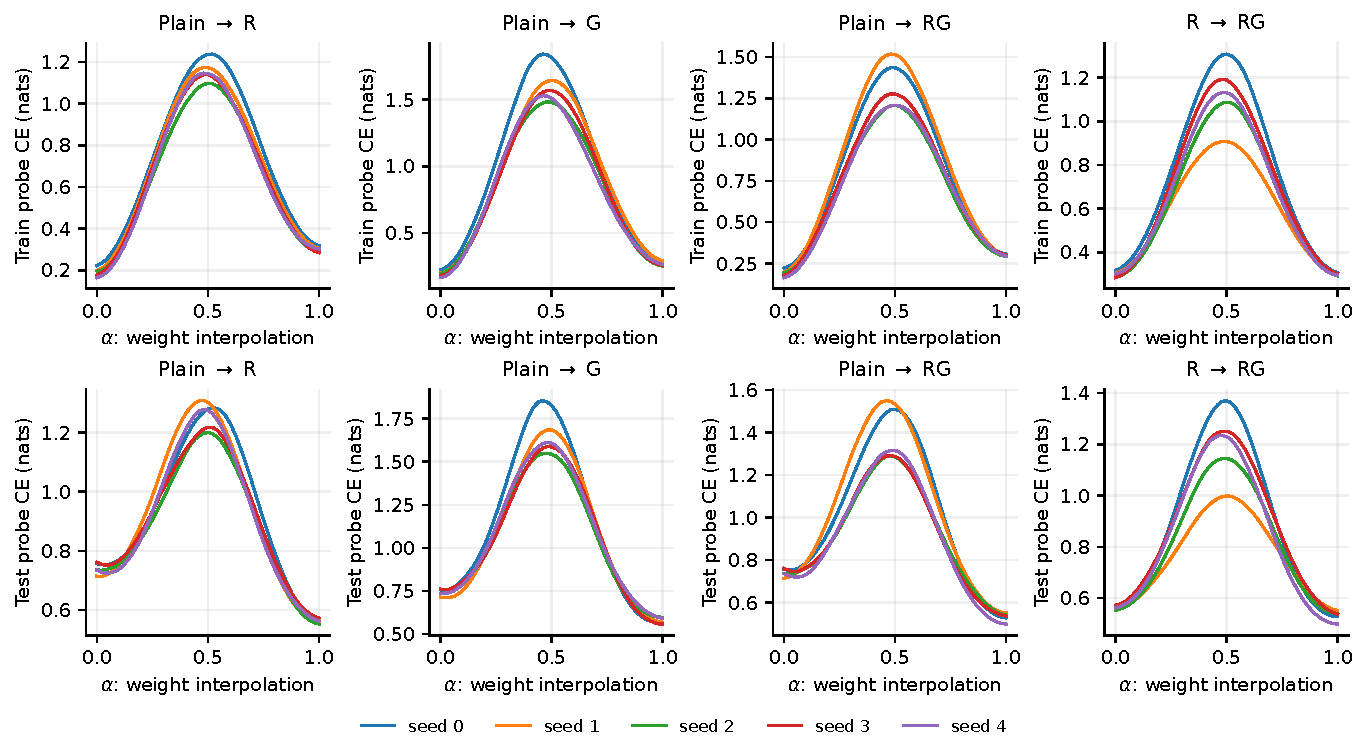
\includegraphics[width=.96\linewidth]{figures/interpolation_summary.pdf}
\caption{Measured straight-segment losses on the training and test probes, with recalibration at every point. Each thin line is one seed. Endpoints correspond to separately trained models, and the horizontal coordinate is interpolation in weights, not training time. Barriers do not establish disconnected basins.}
\label{fig:interpolation}
\end{figure}

PCA summarizes the recorded weight trajectory rather than selecting random directions \citep{li2018visualizing}. In the shared four-method analysis, the first two components explain only $\tPcaTwoLow$--$\tPcaTwoHigh\%$ of the centred checkpoint variance across seeds; four explain $\tPcaFourLow$--$\tPcaFourHigh\%$. Large individual projection errors remain in two dimensions. A checkpoint's projected location on a plotted plane is consequently not the checkpoint itself, and the plane's CE at that location is not its measured CE. Connecting recorded checkpoints also does not recover the unobserved optimization path between them. We retain these projections as diagnostics and do not use them as the main evidence for a geometric mechanism.
